\subsection{Accelerometeralgoritme}\label{sec:imp_vinkler}
I \autoref{sec:test_acc} fremgår det, at der er lineær tendens mellem vinkel og spænding. Det er muligt at udføre en lineær interpolation over dataen af målinger fra accelerometrene i forskellige vinkler. På denne måde er det muligt at bestemme en vinkel for en tilsvarende spænding. En ligning af lineær interpolation fremgår af \autoref{eq:interpolation}.
%Da målingerne af linearitet, målt i \autoref{sec:test_acc}, er foretaget med Ni USB-6009 stemmer spændingerne ikke overens, når det samples på mikrokontrolleren. Dette gør det ikke, da Ni USB-6009 og mikrokontrolleren har forskellige arbejdsområder,
\begin{equation} \label{eq:interpolation}
y=y_{0}+(y_{1}-y_{0})\dfrac{x-x_{0}}{x_{1}-x_{0}}
\end{equation}

\noindent
Af formlen defineres $y_0$ og $y_1$ intervallet af grader for interpolationen, hvor $x_0$ og $x_1$ er de tilhørende samplede spændinger fra acceleromtrene for de målte y-værdier.   

Da der til kontrolsystemet anvendes en anden ADC end i \autoref{sec:test_acc}, udføres nye målinger for at undersøge relationen mellem spænding og vinkel.  
Efterfølgende er der aflæst et offset, som er trukket fra signalet, for at centrere dette omkring 0. Offsettet for accelerometret placeret parallelt med femur er aflæst til et digitalt output på $1.002$, hvilket svarer til et offset på $1,6162~V$. Accelerometret placeret parallelt med tibia er aflæst til $972$, svarende til et offset på $1,5743~V$. De digitale outputs er omregnet til en spænding (U) ved \autoref{eq:vinkler}, hvor $3,3~V$ er forsyningsspændingen, og $2^{11}$ er ADC'ens opløsning målt i bit.  

\begin{equation}
\label{eq:vinkler}
U = digitalt~output\cdot \dfrac{3,3~V}{2^{11}}
\end{equation}

\noindent
Resultaterne for de nye målinger fremgår af \autoref{tab:vinkelinterval_psoc}, hvor det konverterede output for accelerometrene placeret parallelt med henholdsvis femur og tibia er angivet som en vinkel på 0, 10, 30, 50, 70, 80 og $90^{\circ}$. 

\begin{table}[H]
\centering
\begin{tabular}{|c|c|c|}
\hline
\multicolumn{1}{|l|}{\textbf{Vinkel {[}$^{\circ}${]}}} & \textbf{\begin{tabular}[c]{@{}c@{}}Konverterede outputs fra \\ accelerometer placeret \\ parallelt med femur\end{tabular}} & \textbf{\begin{tabular}[c]{@{}c@{}}Konverterede outputs fra \\ accelerometer placeret \\ parallelt med tibia\end{tabular}} \\ \hline
\textbf{0}                                                      & -186                                                                                                     & -179                                                                                                            \\ \hline
\textbf{10}                                                     & -185                                                                                                   & -176
\\ \hline
\textbf{30}                                                     & -168                                                                                                   & -153                                                                                                          \\ \hline
\textbf{50}                                                     & -126                                                                                                  & -111                                                                                                         \\ \hline
\textbf{70} & -76                                                                                                  & -52                                                                                                         \\ \hline
\textbf{80}                                                     & -31                                                                                                  & -16                                                                                                         \\ \hline
\textbf{90}                                                     & 0
& 0
\\ \hline
\end{tabular}
\caption{Konverterede outputs fra accelerometrene placeret parallelt med henholdsvis femur og tibia svarende til givne vinkler.}
\label{tab:vinkelinterval_psoc}  
\end{table}

\noindent
Ud fra de målte værdier i \autoref{tab:vinkelinterval_psoc}, er der opstillet en funktion, der indeholder \textit{ifelse}-løkker, som gør det muligt at vurdere, hvilket interval en given spænding befinder sig indenfor. 
I hver løkke anvendes lineær interpolation, som har til opgave at finde en vinkel, der er svarende til en spænding, som ligger mellem et interval og returnerer denne. 

Når der er udført lineær interpolation over dataen skal de målte accelerometerdata lægges sammen for at få den samlede vinkel over knæet. 
Ved at implementere værdierne fra \autoref{tab:vinkelinterval_psoc} i mikrokontrolleren kan signalet repræsenteres som en samlet vinkel af knæet. Af \autoref{fig:acc_imp} fremgår vinklen over knæet ved udførelse af en squat-øvelse.
 

\begin{figure}[H]
\centering
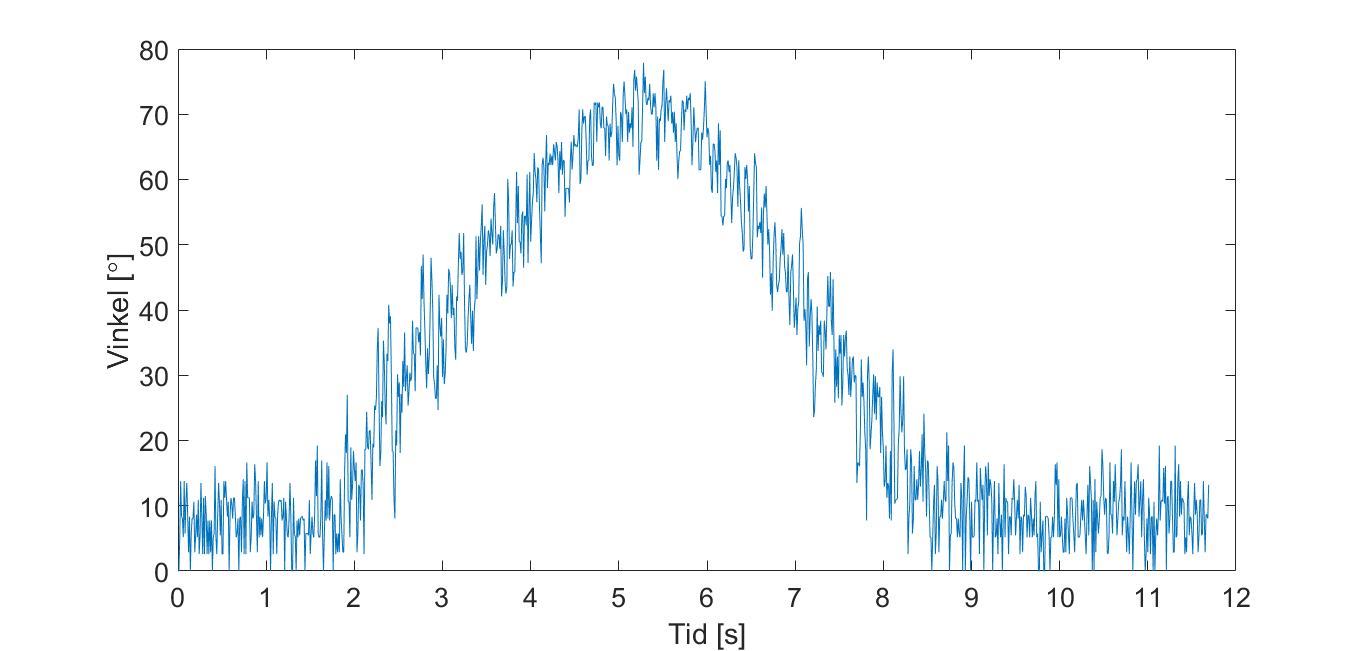
\includegraphics[width=1\textwidth]{figures/Pilotforsoeg/accvinkel}
\caption{Vinklen over knæet under udførelsen af en squat-øvelse.}
\label{fig:acc_imp}
\end{figure}



